\documentclass[final]{article}

\usepackage{APS360}
\usepackage[utf8]{inputenc}
\usepackage[T1]{fontenc}
\usepackage{hyperref}
\usepackage{url}
\usepackage{booktabs}
\usepackage{amsfonts}
\usepackage{nicefrac}
\usepackage{microtype}
\usepackage{xcolor}
\usepackage{graphicx}
\usepackage{tikz}
\usetikzlibrary{positioning, arrows.meta, fit, backgrounds}
\renewcommand{\arraystretch}{0.88}
\setlength{\abovecaptionskip}{3pt}
\setlength{\belowcaptionskip}{0pt}

\title{Mini-VLM: Progress Report}

\author{%
  Oliver Petrovic \\
  1008923042, oliver.petrovic@mail.utoronto.ca\\
  \url{https://github.com/Olipet24/mini-vlm}\\
}

\begin{document}

\maketitle

\vspace{-0.5in}

\section*{Introduction}

Modern Vision-Language Models (VLMs) are massive, requiring billions of parameters and huge GPU
resources that make them impossible to run on everyday or mobile hardware. Mini-VLM is a compact
VLM for Visual Question Answering (VQA) constrained to a strict \textbf{100MB storage budget},
targeting edge deployment: given a $224\times224$ image and a free-form text question, the model
outputs one of the 1000 most common VQA answers (Figure~\ref{fig:pipeline}). Running AI models on
resource-constrained hardware requires aggressive compression, and mapping raw pixels and
free-form text jointly onto a correct answer requires learned, non-linear visual and linguistic
representations that hand-coded rules cannot approximate (Goyal et al., 2017), which is why deep
learning is appropriate here. Rather than shrinking a Transformer-based VLM post hoc, our core
contribution is a \emph{unified RWKV pipeline}: an RWKV spatial bridge and RWKV language core
replace attention everywhere, giving linear-time (not quadratic) cost in the combined visual+text
sequence length (Peng et al., 2023), instead of the linear-projector-into-attention approach used
by connectors such as LLaVA (Liu et al., 2023). Figure~\ref{fig:pipeline} also shows our
control-group baseline, which keeps the same frozen encoder but replaces the RWKV bridge/core
with a linear projector and a standard Transformer, isolating the RWKV design's contribution.

\begin{figure}[!htbp]
  \centering
  \resizebox{\linewidth}{!}{%
  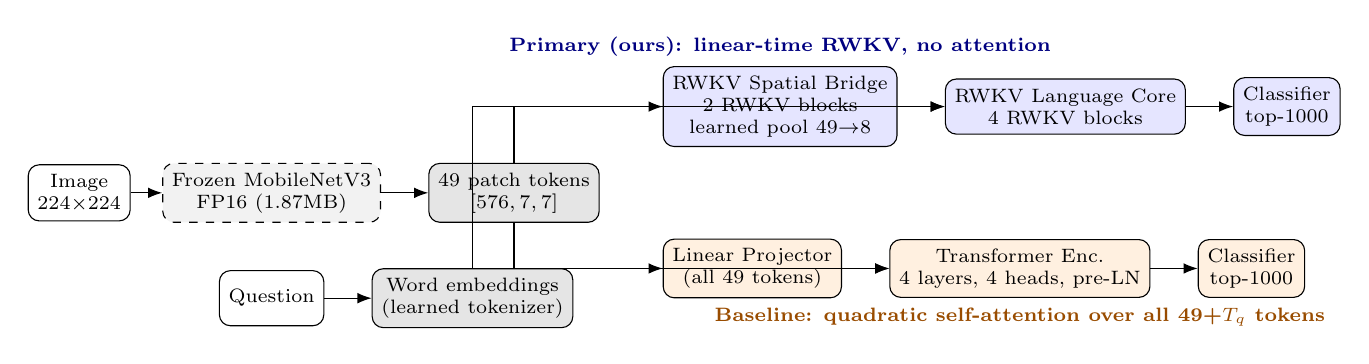
\begin{tikzpicture}[
      node distance=4mm and 4mm,
      box/.style={draw, rounded corners, align=center, minimum height=0.7cm, font=\scriptsize},
      frozen/.style={box, dashed, fill=gray!10},
      primary/.style={box, fill=blue!10},
      base/.style={box, fill=orange!12},
      shared/.style={box, fill=gray!20},
      arr/.style={-{Latex[length=1.8mm]}}
    ]
    \node[box] (img) {Image\\$224{\times}224$};
    \node[frozen, right=of img] (enc) {Frozen MobileNetV3\\FP16 (1.87MB)};
    \node[shared, right=6mm of enc] (tok) {49 patch tokens\\$[576,7,7]$};
    \node[box, below=6mm of enc] (q) {Question};
    \node[shared, right=6mm of q] (qtok) {Word embeddings\\(learned tokenizer)};

    \node[primary, above right=2mm and 8mm of tok] (bridge) {RWKV Spatial Bridge\\2 RWKV blocks\\learned pool $49{\to}8$};
    \node[primary, right=6mm of bridge] (core) {RWKV Language Core\\4 RWKV blocks};
    \node[primary, right=6mm of core] (ans1) {Classifier\\top-1000};

    \node[base, below right=2mm and 8mm of tok] (proj) {Linear Projector\\(all 49 tokens)};
    \node[base, right=6mm of proj] (xfmr) {Transformer Enc.\\4 layers, 4 heads, pre-LN};
    \node[base, right=6mm of xfmr] (ans2) {Classifier\\top-1000};

    \draw[arr] (img) -- (enc);
    \draw[arr] (enc) -- (tok);
    \draw[arr] (tok) |- (bridge);
    \draw[arr] (tok) |- (proj);
    \draw[arr] (bridge) -- (core);
    \draw[arr] (core) -- (ans1);
    \draw[arr] (proj) -- (xfmr);
    \draw[arr] (xfmr) -- (ans2);
    \draw[arr] (q) -- (qtok);
    \draw[arr] (qtok) |- (core.west);
    \draw[arr] (qtok) |- (xfmr.west);

    \node[font=\scriptsize\bfseries, blue!50!black, above=0mm of bridge] {Primary (ours): linear-time RWKV, no attention};
    \node[font=\scriptsize\bfseries, orange!60!black, below=0mm of xfmr] {Baseline: quadratic self-attention over all 49+$T_q$ tokens};
  \end{tikzpicture}%
  }
  \caption{Implemented pipeline for both models. The frozen vision encoder runs once, offline,
  and its FP16 features are cached; only the bridge/projector and language core/Transformer are
  trained. The primary model compresses 49 spatial tokens to 8 language-aligned tokens with a
  learned pooling matrix before its shared RWKV stack; the baseline instead feeds all 49 tokens
  into a standard multi-head-attention Transformer, so the comparison isolates the RWKV bridge's
  contribution rather than encoder or data differences.}
  \label{fig:pipeline}
\end{figure}

\section*{Data Processing}

We use the official \textbf{VQA v2.0} dataset (questions/annotations over COCO images), cleaned
in two steps to fit a 100MB budget: (1) collapse free-form answers to a \textbf{top-1000
most-common-answer classification} problem, built from the frequency distribution over the full
443{,}757-example train2014 pool (87.47\% coverage), dropping examples outside that vocabulary;
(2) resize/normalize images to $224\times224$ and pass them through the frozen vision encoder
\emph{once, offline}, caching the resulting $576\times7\times7$ FP16 feature map so training
never re-runs the CNN. All numbers below are the full, production-scale run
(Table~\ref{tab:stats}); a small CPU-only subset was used only for early development.

\begin{table}[!htbp]
\centering
\footnotesize
\begin{tabular}{lr}
\toprule
Statistic & Value \\
\midrule
Train / val / test size & 368{,}751 / 19{,}407 / 186{,}489 \\
Unique images (train+val; test) & 82{,}575; 40{,}404 \\
Cached FP16 feature tensors & 122{,}979 \\
Answer-type mix (yes/no : other : number) & 43.1\% : 43.5\% : 13.4\% \\
Question length (words), mean [min, max] & 6.1 [2, 22] \\
Top-1000 answer coverage (train2014 pool) & 87.47\% \\
\bottomrule
\end{tabular}
\caption{Full-scale dataset statistics (\texttt{outputs/processed\_full/dataset\_stats.json}).}
\label{tab:stats}
\end{table}

\textbf{Train/val/test split.} \texttt{train}/\texttt{val} are disjoint samples from the
official \emph{train2014} pool; \texttt{test} is sampled entirely from \emph{val2014} -- images
and questions never seen during training or hyperparameter selection, our stand-in for
``never-before-seen'' data at this stage. For final testing we plan to submit predictions to the
official blind VQA v2.0 \emph{test2015} evaluation server, whose answers are not public.

\textbf{Example cleaned sample.} Figure~\ref{fig:sample} shows one training example after
cleaning: image, question, and the multiple-choice answer used as the classification target.

\begin{figure}[!htbp]
  \centering
  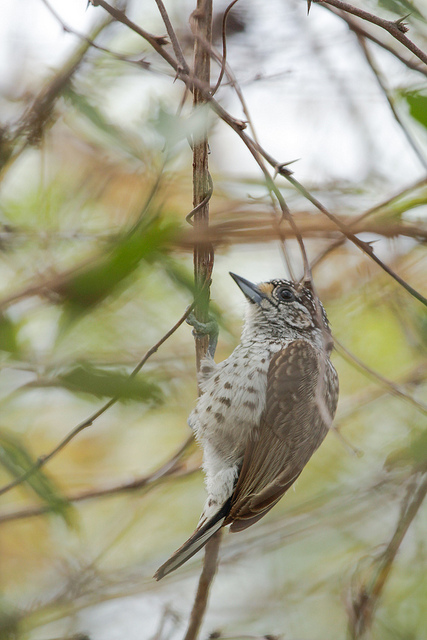
\includegraphics[height=2.0cm]{figures/sample_bird.jpg}
  \caption{Cleaned training example. Question: ``What color is this bird?'' Target answer
  (class \texttt{white and brown}, one of the top-1000 answer classes).}
  \label{fig:sample}
\end{figure}

\textbf{Challenges.} Downloading/extracting the full $\sim$123,000-image COCO zip archives once
was more reliable than the CPU-subset's per-image fetches, but not error-free: a batch of cached
feature tensors was silently corrupted, spiking training loss until we added a feature-integrity
check (\texttt{mini\_vlm/data/check\_features.py}) that now runs before training.

\section*{Baseline Model}

The baseline is the ``naive integration'' control group from the proposal: the same frozen
vision encoder, but a plain \textbf{Linear Projector} maps all 49 spatial patch tokens (no
compression) into a standard, unshared \texttt{nn.TransformerEncoder} (4 layers, 4 heads,
$d_{model}=128$, pre-LN, Figure~\ref{fig:pipeline}) alongside the question's word embeddings;
the final token's hidden state is classified into 1000 answers, no tuning beyond standard
defaults (AdamW, $lr=3\times10^{-3}$).

\textbf{Quantitative results.} Trained for 10 epochs ($587.9$s $\approx$9.8 min) on the full
training pool, the baseline reaches \textbf{47.38\%} held-out test accuracy (2{,}574{,}696
params, 9.84MB) against a \textbf{21.84\%} majority-class floor (Table~\ref{tab:comparison});
validation loss is still falling at epoch 10 (1.89$\to$1.55), i.e.\ not yet overfitting.

\textbf{Qualitative results.} Table~\ref{tab:qualitative} (``baseline'' column) shows
representative predictions. Early on, an unshared Transformer trained from scratch was fragile
-- post-LN produced loss spikes/NaNs, fixed via pre-LN -- and collapsed to one high-frequency
answer regardless of question; the trained model now gives varied, sometimes low-confidence
answers, doing best on open-ended ``other'' questions (Table~\ref{tab:comparison}).

\section*{Primary Model}

\textbf{Vision Encoder.} Frozen, pretrained MobileNetV3-Small, compressed FP32$\to$FP16 (3.66MB
$\to$ 1.87MB). INT8 post-training static quantization hit an operator-support gap instead
(MobileNetV3's Squeeze-and-Excite blocks need a quantized elementwise multiply unimplemented in
this environment's quantized-CPU kernels); FP16 is a reliable substitute, INT8/GPTQ (Frantar et
al., 2023) a concrete next step.

\begin{table}[!htbp]
\centering
\footnotesize
\resizebox{\linewidth}{!}{%
\begin{tabular}{lrrrrrrr}
\toprule
Model & Params & Size & Test acc. & Test loss & Acc.\ y/n & Acc.\ other & Acc.\ num.\\
\midrule
Majority-class floor & -- & -- & 21.84\% & -- & -- & -- & -- \\
Baseline (Linear + Transformer) & 2{,}574{,}696 & 9.84MB & \textbf{47.38\%} & \textbf{1.60} & 57.57\% & \textbf{42.81\%} & \textbf{29.35\%} \\
\textbf{Primary (RWKV bridge + core)} & 3{,}069{,}680 & 11.75MB & 46.70\% & 1.91 & \textbf{59.68\%} & 39.30\% & 28.88\% \\
\bottomrule
\end{tabular}%
}
\caption{Baseline vs.\ primary, full-scale test set (186{,}489 questions: 80{,}539 yes/no,
80{,}930 other, 25{,}020 number), 10 epochs each, same optimizer/data/seed. Best per column
bolded.}
\label{tab:comparison}
\end{table}

\textbf{RWKV Spatial Bridge (our main contribution).} RWKV time-mixing (WKV linear-time
recurrence, custom CUDA kernel for GPU) and channel-mixing (squared-ReLU FFN), from scratch --
no attention. It flattens the $576\times7\times7$ feature map into 49 tokens, projects to
$d_{model}=128$, runs 2 RWKV blocks, then compresses to 8 language-aligned tokens via a
\emph{learned linear pooling matrix} ($8\times49$ softmax-normalized weights, not cross-attention).

\textbf{RWKV Language Core.} The 8 visual tokens concatenate with question word embeddings and
pass through a 4-layer RWKV stack (dropout 0.1 throughout); the final hidden state feeds a linear
classifier over 1000 answers. Total: \textbf{3{,}069{,}680 parameters}, 11.75MB state dict --
combined with the 1.87MB FP16 vision encoder, a \textbf{13.62MB} deployed model, $\approx$86MB of
headroom left in the budget.

\begin{figure}[!htbp]
  \centering
  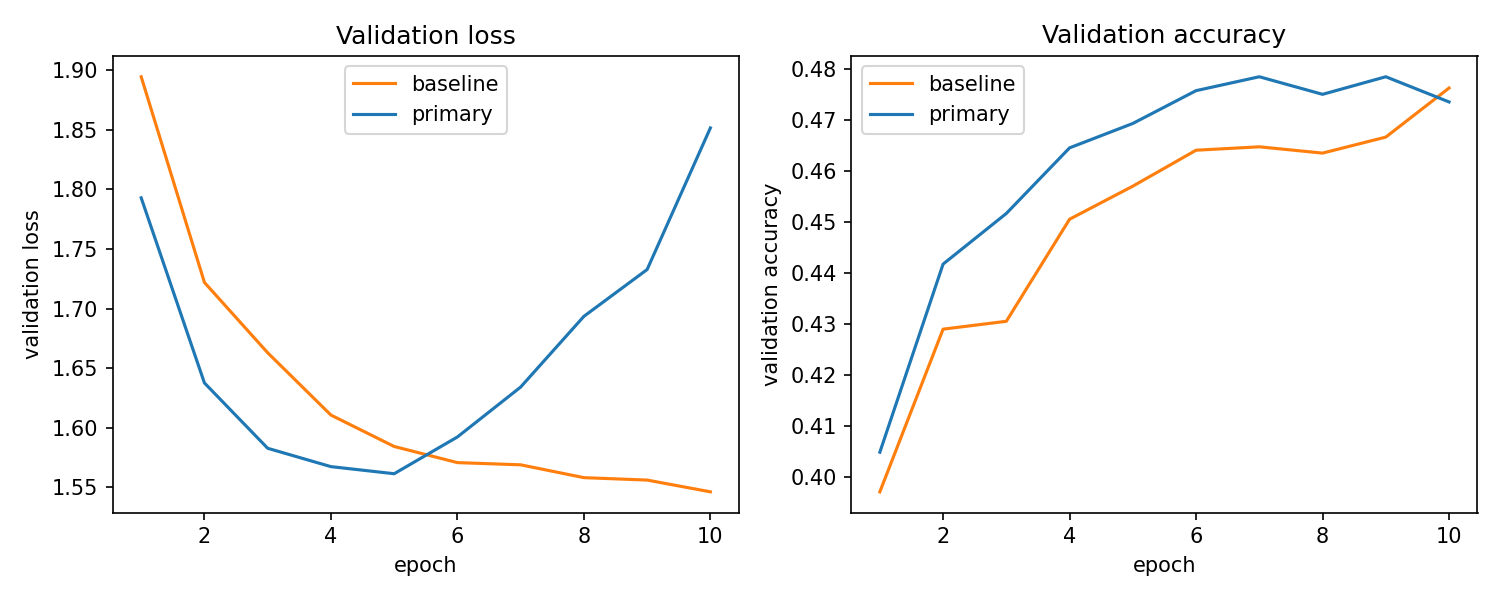
\includegraphics[width=0.46\linewidth]{figures/comparison_curves.png}
  \caption{Baseline vs.\ primary validation loss/accuracy, full-scale run, 10 epochs. Primary's
  validation loss bottoms around epoch 5 then climbs back to 1.85 by epoch 10 even with dropout
  active throughout; the baseline's is still falling at epoch 10 -- primary overfits earlier and
  more despite having only $\sim$20\% more parameters.}
  \label{fig:comparison_curves}
\end{figure}

\textbf{Quantitative results.} Overall test accuracy is essentially tied (46.70\% vs.\ 47.38\%),
but the per-type breakdown (Table~\ref{tab:comparison}) is more specific: primary is
\emph{better} on yes/no (59.68\% vs.\ 57.57\%), where 8 compressed tokens carry enough coarse
scene information for a binary decision, but \emph{worse} on open-ended ``other'' (39.30\% vs.\
42.81\%), where the baseline's uncompressed 49 tokens and full self-attention keep fine-grained
detail the bridge's pooling discards. Both are tied and weakest on counting (29.35\% vs.\
28.88\%) -- a data/architecture-agnostic limitation, not one the compression specifically causes.

\textbf{Qualitative results.} Table~\ref{tab:qualitative} shows the same held-out questions for
both models. When primary is right on a yes/no question it is confident (e.g.\ ``bird to land?'',
0.74 vs.\ baseline's wrong 0.65 for ``no''); on harder ``other'' questions it can be confidently
wrong (ground truth \emph{apple}, primary predicts \emph{hat} at 0.77) -- consistent with a
frozen encoder and 8 compressed tokens losing detail needed to localize a small object.

\begin{table}[!htbp]
\centering
\footnotesize
\resizebox{\linewidth}{!}{%
\begin{tabular}{lccc}
\toprule
Question (truth, type) & Baseline pred. & Primary pred. \\
\midrule
Wearing a shirt? (no, y/n) & yes (0.68) & \textbf{no (0.51)} \\
Somewhere for bird to land? (yes, y/n) & no (0.65) & \textbf{yes (0.74)} \\
How many signs in picture? (3, num) & 1 (0.26) & 1 (0.52) \\
What color is the shirt? (white, other) & \textbf{white (0.80)} & blue (0.35) \\
What object is behind the women? (apple, other) & frisbee (0.73) & hat (0.77) \\
\bottomrule
\end{tabular}%
}
\caption{Representative held-out predictions, conf.\ in parens (correct bolded), full-scale
checkpoints (full set + image grid in \texttt{outputs/results\_full/}).}
\label{tab:qualitative}
\end{table}

\textbf{Challenges \& feasibility.} The WKV recurrence's stable form (Peng et al., 2023) needed
care to avoid overflow; we verified the CUDA kernel against the pure-Python reference on GPU
(max diff.\ $<10^{-6}$, \texttt{verify\_wkv\_cuda.py}) before trusting it. Dropout was already
active here, yet primary still overfits earlier/further than the baseline
(Figure~\ref{fig:comparison_curves}) -- a best-val checkpoint or stronger regularization is a
concrete next step. Feasibility: the full pool (368{,}751 examples) trains both models in under
10 min.\ each on one GPU, beating the 21.84\% majority floor by $\approx$25 points at
$\le$13.62MB, well inside the 100MB budget.

\newpage
\section*{References}
Goyal, Y., Khot, T., Summers-Stay, D., Batra, D., \& Parikh, D. (2017). Making the V in VQA
Matter: Elevating the Role of Image Understanding in Visual Question Answering. \emph{CVPR}.

Peng, B., et al. (2023). RWKV: Reinventing RNNs for the Transformer Era. \emph{EMNLP}.

Liu, H., Li, C., Wu, Q., \& Lee, Y. J. (2023). Visual Instruction Tuning. \emph{NeurIPS}.

Frantar, E., Ashkboos, S., Hoefler, T., \& Alistarh, D. (2023). GPTQ: Accurate Post-Training
Quantization for Generative Pre-trained Transformers. \emph{ICLR}.

\end{document}
